\chapter{Surveying The Active Divergence Landscape}
\label{ch:active_div}

\section{Introduction}

This chapter is an updated version of the survey paper and taxonomy of active divergence methods that I presented at the International Conference on Computational Creativity (ICCC) in 2021 \citep{broad2021active} in collaboration with Sebastian Berns and Simon Colton from Queen Mary, University of London. 
The concept of active divergence was introduced by \cite{berns2020bridging} at ICCC the year before, and this survey is a follow-up to that first introduction of active divergence, giving a comprehensive account of all active divergence methods that were published and disseminated in 2021. 
This survey and taxonomy was developed primarily by myself, and Berns and Colton were brought on as collaborators later in the process, to get their insights into this, and get their perspective on the survey from the perspective of computational creativity research, which is the primary community that this survey was first disseminated in.

Much like the \cite{berns2020bridging} paper, this survey bridges together two related but distinct fields of AI research and creative practice: CreativeAI research and computational creativity \citep{cook2018neighbouring}.
Many of the novel advances in this survey are presented from creative practitioners working in the CreativeAI communities, where work is primarily shared in the NeurIPS Workshop on Machine Learning for Creativity and Design, as well as developments being shared on social media and open-source code channels like twitter, github, and colab notebooks. 
A great deal of effort was made on my part to find and document the original contributions, regardless of where they were disseminated, so as not to just rely on peer-reviewed machine learning and computational creativity papers, which would have given only a partial view of the developments in this space when the CreativeAI community was flourishing between 2017-2021.

All of the work from the experimental work in this thesis from Chapters \ref{ch:unstable_eq}, \ref{ch:divergent} \& \ref{ch:net_bend} are presented in this survey and taxonomy.
It is unconventional to present a survey at the end of the thesis, and include the work done by the author in the survey, but to exclude my own contributions in this survey would give an incomplete picture of the active divergence landscape, given that the three chapters of experimental work in this thesis are each three different categorical contributions to active divergence methods.
I also decided to put this survey at the end of the thesis to better reflect the timeline of events, much of the work by others in active divergence happened concurrently with my own work, so would have given a misleading chronology if this were to have all been documented in the background chapter of this thesis (Chapter \ref{ch:background}). 
Any works that precede this thesis are also documented in the background chapter (\S \ref{c2:sec:data-divergent}), but presented again here in the context of the wider developments in this survey and taxonomy. 
This survey starts with a statistical view of standard generative model training and then proceeds onto the many different ways that active divergence can be achieved in relation to this statistical view.
The divergence in active divergence, refers to the statistical definition of divergence, as the distance between two data distributions, and should not be confused with other definitions of divergence such as divergent thinking from psychology and creativity research \citep{guilford1957creative}.

\section{Generative Models: A Statistical View}

While not all generative models rely on generative deep learning, this survey focuses on models built with artificial neural networks\footnote{
    For further reading, a comprehensive overview of generative models is given in \citet{harshvardhan2020comprehensive}.}. 
Given a data distribution $P$, a generative model will model an approximate distribution $P'$. 
The parameters for the approximate distribution can be learned by an artificial neural network. 
This learning task is tackled differently by different architectures and training schemes. 
E.g. autoencoders \citep{rumelhart1985learning} and variational autoencoders (VAE) \citep{kingma2013auto,rezende2014stochastic} learn to approximate the data through reconstruction via an encoding and a decoding network, while generative adversarial networks (GAN) \citep{goodfellow2014generative} consists of a generator that is guided by a discriminating network. 
In most cases, the network learns a mapping from a lower-dimensional latent distribution $X$ to the complex high-dimensional feature space of a domain. 
The model, thus, generates a sample $p'$ given an input vector $x$ which should resemble samples drawn from the target distribution $P$. 
In the simplest case of a one-layer network the generated sample $p'$ is generated using the function: $p' = \sigma(Wx+b)$ where $x$ is the input vector from the latent distribution $x \in X$, $\sigma$ is a non-linear activation function, $W$ and $b$ are the learned association matrix and bias vector for generating samples in the approximate distribution $p' \in P'$. 
The model parameters $W$ and $b$, are typically learned through a gradient-based optimisation process. 
In this process, a loss function will require the model to maximise the likelihood of the data either: (i) explicitly, as in the case of autoencoders, and autoregressive models \citep{frey1996does}; (ii) approximately, as is the case in VAEs; (iii) or implicitly, as in the case of GANs. Generative models can also be conditioned on labelled data. In the conditional case, the generative model takes two inputs $x$ and $y$, where $y$ represents the class label vector. 
Another form of conditional generative models is translation models, such as pix2pix \citep{isola2017image}, that takes a (high dimensional) data distribution as input $Q$ and learns a mapping to $P'$ which is an approximation of the true target function $f: Q \rightarrow P$.

\begin{figure}[!htbp]
    \centering
    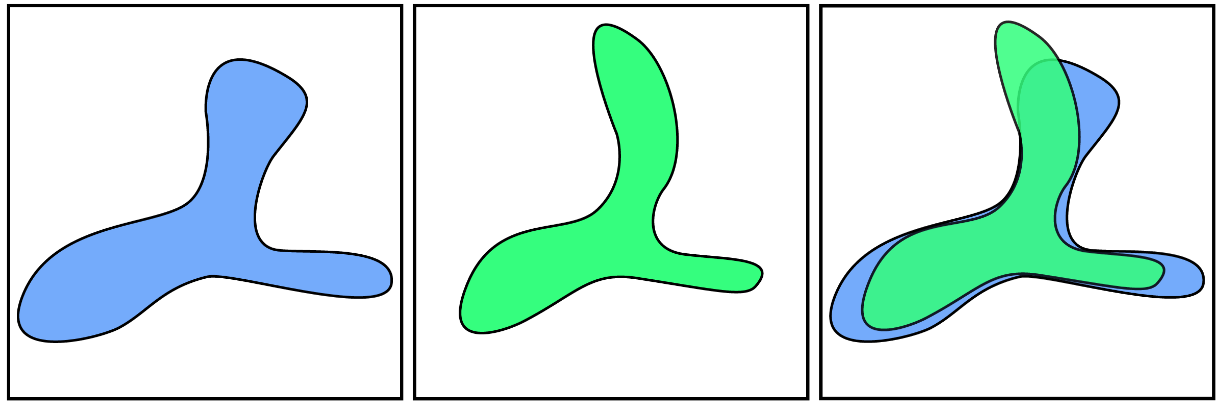
\includegraphics[width=1\textwidth]{figures/c2_background/diagrams/training_gen_model_distro_view.png}
    \caption[Diagram illustrating the distribution view of training a generative model.]{Diagram illustrating the parameter view of training a generative model. \textbf{Left:} The true distribution \textcolor{blue}{$P$}. \textbf{Middle:} The approximate distribution \textcolor{green}{$P'$}. \textbf{Right:} The approximate distribution \textcolor{green}{$P'$} overlayed on the true distribution \textcolor{blue}{$P$}.}
  \label{fig:c6:gen-model-distribution-view}
  \end{figure}

\begin{figure}[!htbp]
    \centering
    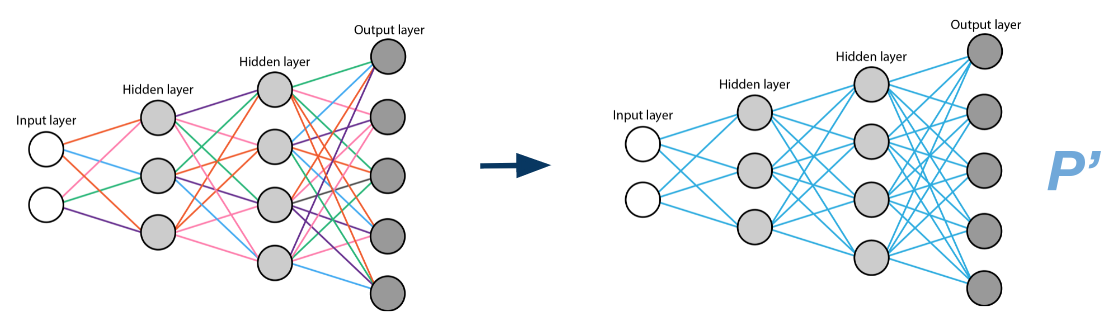
\includegraphics[width=1\textwidth]{figures/c2_background/diagrams/training_generative_model_parameter_view.png}
    \caption[Diagram illustrating the parameter view of training a generative model.]{Diagram illustrating the parameter view of training a generative model. A network with randomly initialised parameters is trained to model the true distribution $P$ and produces the approximate distribution \textcolor{blue}{$P'$}}.
  \label{fig:c6:gen-model-parameter-view}
  \end{figure}

All deep generative models, and in particular ones that generate high dimensional data domains like images, audio and natural language, will have some level of divergence $D(P||P') \geq 0$ between the target distribution $P$ and the approximate distribution $P'$, because of the complexity and stochasticity inherent in high dimensional data. 
The goal of all generative models is to minimise that level of divergence, by maximising the likelihood of generating the given data domain. 
Active divergence methods, however, intentionally seek to create a new distribution $U$ that does not directly approximate a given distribution $P$, or resemble any other known data distribution. 
This is either done by seeking to find model parameters $W^*$ and $b^*$ (in the single layer case) that generate novel samples $u = \sigma(W^*x+b^*)$ or by making other kinds of interventions to the chain of computations.

\section{Taxonomy of Active Divergence Methods}
\label{c6:sec:taxonomy}

This section presents the taxonomy and survey of active divergence methods. 
For three of these categories of active divergence methods, I have made major contributions, being the first to publish examples of all of these methods, (detailed in Chapters \ref{ch:unstable_eq}, \ref{ch:divergent} \& \ref{ch:net_bend}).
This section will reiterate these contributions, for the purposes of defining, formally explaining and delineating them from other approaches.

\subsection{Novelty Search Over Learned Representations}
\label{survey:noveltysearch}

\begin{figure}[!htbp]
    \centering
    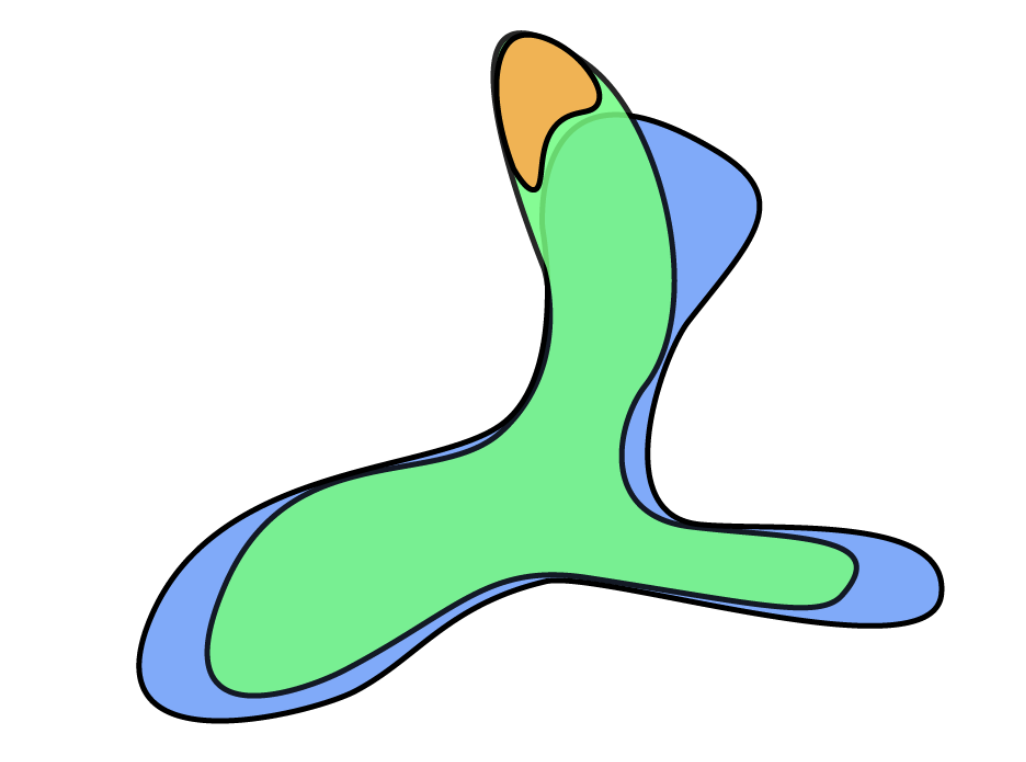
\includegraphics[width=1\textwidth]{figures/c6_active_div/diagrams/novelty_search.png}
    \caption[Diagram illustrating the distribution view of novelty search over learned representations.]{Diagram illustrating the distribution view of novelty search over learned representations which finds the subset \textcolor{orange}{$U$} of the approximate distribution \textcolor{green}{$P'$} that is not present in true distribution \textcolor{blue}{$P$}.}
  \label{fig:c6:novelty-search}
  \end{figure}

Methods in this category take existing generative models trained using standard maximum likelihood regimes and then specifically search for the subset of learned representations that do not resemble the training data by systematically sampling from the model. 
Taking account of the fact that any approximate distribution $P'$ will be somewhat divergent from the true distribution $P$, these methods seek to find the subset $U$ of the approximate distribution which is not contained in the true distribution $U \subset P' \wedge U \not\subset P$. \citet{kazakcci2016digits} present an algorithm for searching for novelty in the latent space of a sparse autoencoder trained on the MNIST dataset \citep{lecun1998gradient}. 
They start by creating a sample of random noise and by using a Markov chain Monte Carlo (MCMC) method of iteratively re-encoding the sample through the encoder, then refining the sample until it produces a stable representation. 
They use this approach to map out all the representations the model can generate, then perform k-means clustering on the latent space encoding of these representations. 
By disregarding clusters that correspond to real digits, they are left with clusters of representations of digits that do not exist in the original data distribution. 
It has been argued that these `spurious samples' are the inevitable outcome of generative models that learn to generalise from given data distributions \citep{kegl2018spurious} and that there is a trade-off between the ability to generalise to every mode in the dataset and the ratio of spurious samples in the resulting distribution. 

\begin{figure}[!htbp]
    \centering
    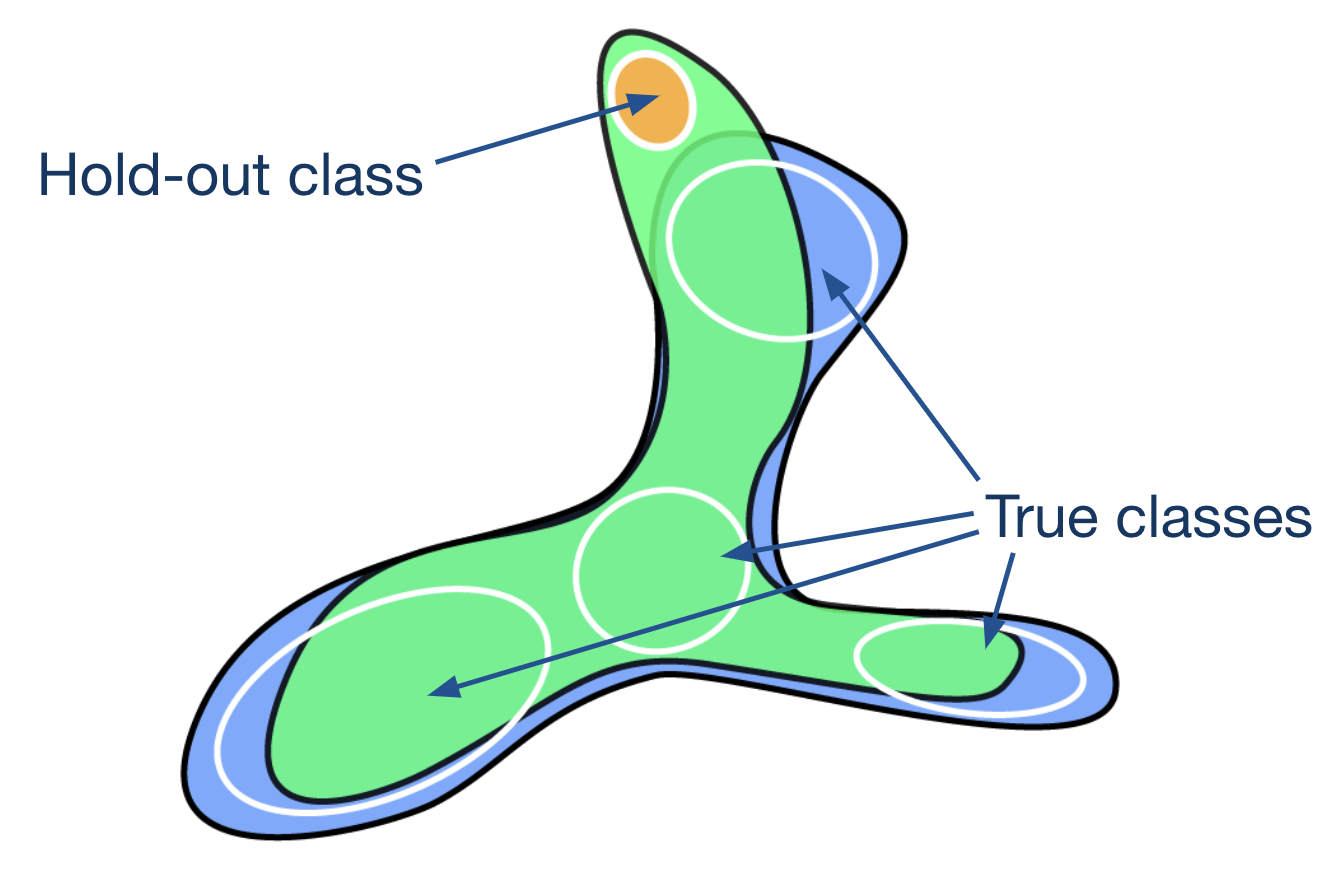
\includegraphics[width=1\textwidth]{figures/c6_active_div/diagrams/hold_out.png}
    \caption[Novelty search over learned representations using hold-out classes]{Diagram illustrating the distribution view of using hold-out classes to encapsulate the subset \textcolor{orange}{$U$} of the approximate distribution \textcolor{green}{$P'$} that is not present in true distribution \textcolor{blue}{$P$}.}
  \label{fig:c6:novelty-search-hold-out}
  \end{figure}

\subsection{Novelty Generation from an Inspiring Set}
\label{survey:noveltygeneration}

The methods in this section train a model from scratch using a training dataset but do not attempt to model the data directly, rather using it as reference material to draw inspiration from. 
We, therefore, refer to this training set (the given distribution $P$) as the inspiring set \citep{ritchie2007some}.

An approach for novel glyph generation utilises a class-conditional generative model trained on the MNIST dataset \citep{lecun1998gradient}, but in this case they train the model with `hold-out classes' \citep{cherti2017out}, additional classes that do not exist in the training data distribution. 
These hold-out classes can then be sampled during inference, which encapsulate the subset $U$ of the approximate distribution $P'$ that is not included in the target distribution $U \subset P' \wedge U \not\subset P$. 
These divergent samples can then be generated directly by conditioning the generator with the hold-out class label, without the need for searching the latent space. 

An approach that directly generates a new distribution $U$ from an inspiring set $P$ is the creative adversarial networks (CAN) algorithm \citep{elgammal2017can}. 
The algorithm uses the WikiArt dataset \citep{saleh2016large}, a labelled dataset of paintings classified by `style' (historical art movement). This algorithm draws inspiration from the GAN training procedure \citep{goodfellow2014generative}, but adapts it such that the discriminator has to classify real and generated samples by style, and the generator is then optimised to maximise the likelihood of the generated results being classified as `artworks' (samples that fit the training distribution of existing artworks) but maximise their deviation from existing styles in order to produce the novel distribution $U$. A similar approach is also taken in \cite{chelma2022creative} with their Bounded Adversarial Divergence (BAD) algorithm for training generative neural networks to diverge from existing labelled classes, but to maintain generated samples within the overall training data distribution.

\begin{figure}[!htbp]
    \centering
    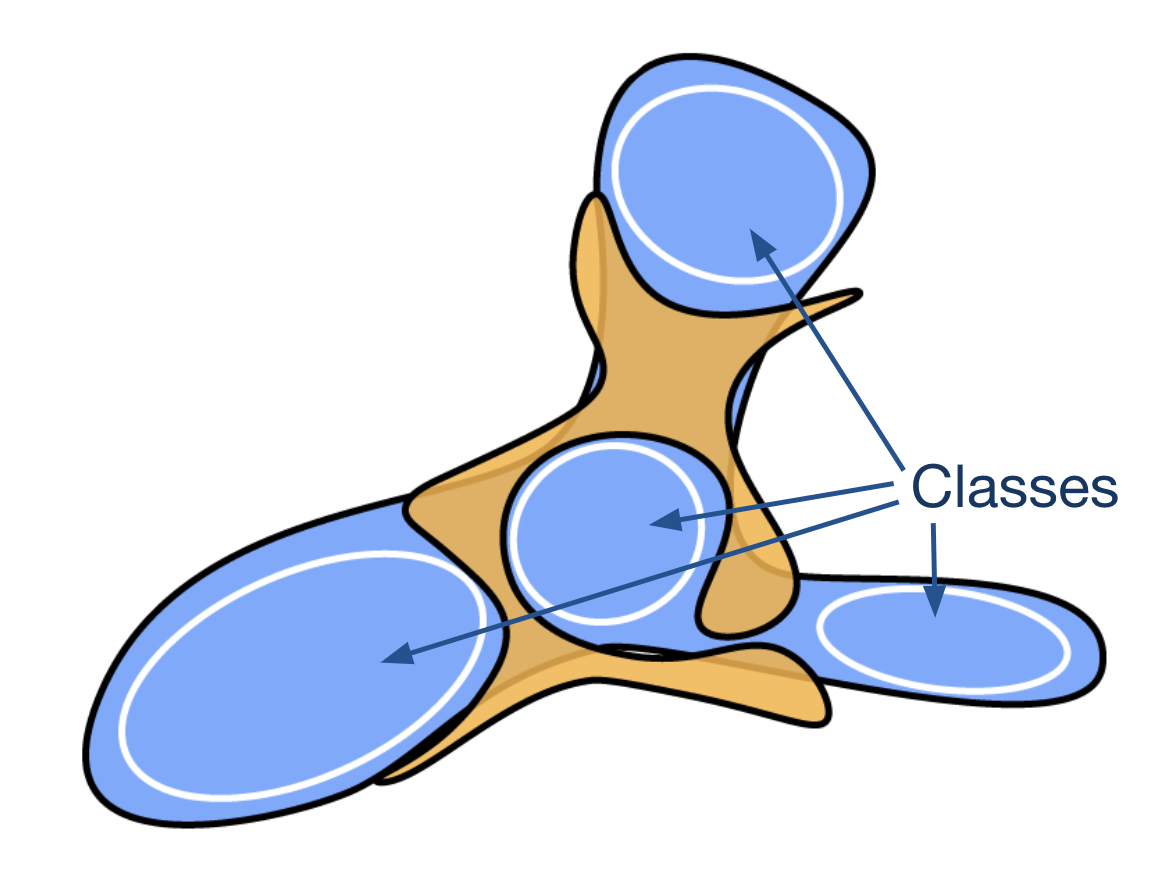
\includegraphics[width=1\textwidth]{figures/c6_active_div/diagrams/creative_adversarial_networks.png}
    \caption[Novelty generation from an inspiring set]{Diagram illustrating novelty generation from an inspiring set, from the distribution view in the creative adversarial networks framework \citep{elgammal2017can} that learns to generate the distribution \textcolor{orange}{$U$} by fitting the true distribution \textcolor{blue}{$P$} which divergence from the existing classes within the distribution}
  \label{fig:c6:novelty-gen-inspiring-set}
  \end{figure}

\subsection{Training Without Data}
\label{survey:nodata}

Training a model from a random initial starting point without any training data almost certainly guarantees novelty in the resulting generated distribution. 
Existing approaches to doing this all rely on the dynamics between multiple models to produce emergent behaviours through which novel data distributions can be generated. 

\begin{figure}[!htbp]
    \centering
    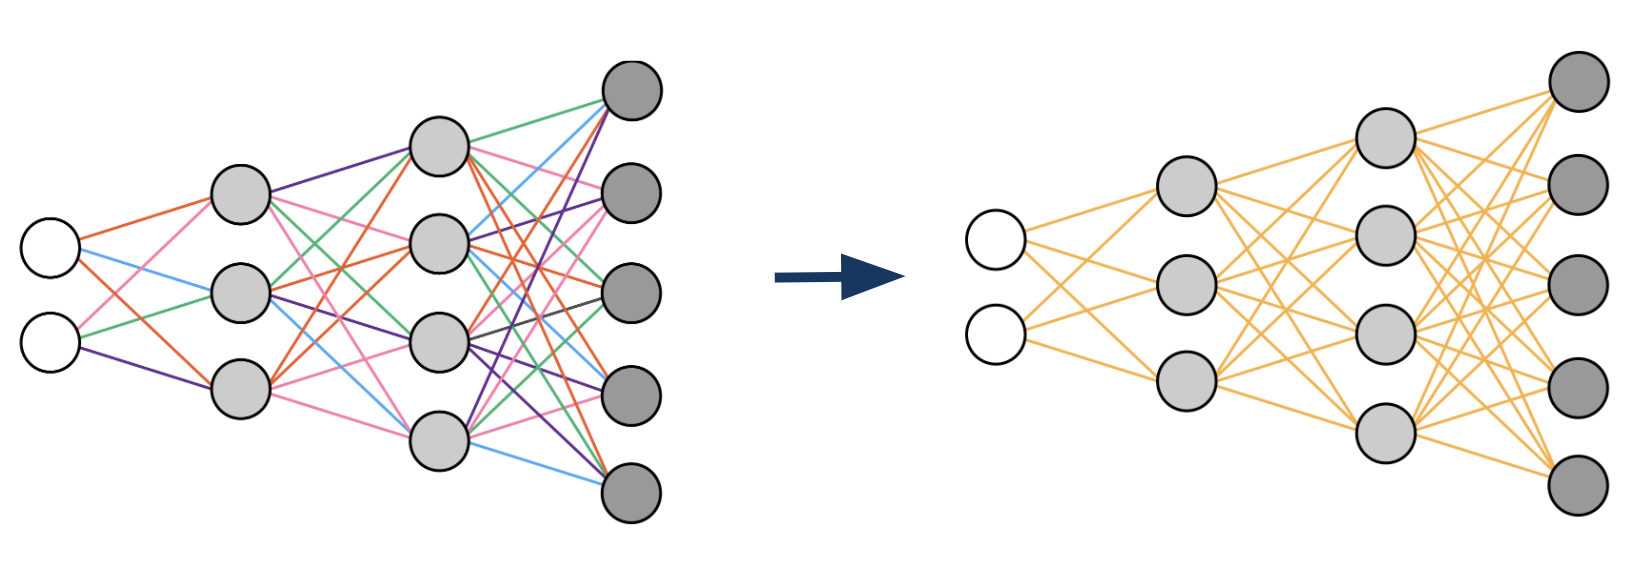
\includegraphics[width=1\textwidth]{figures/c6_active_div/diagrams/training_without_data.png}
    \caption[Diagram illustrating the network parameter view of training without data.]{Diagram illustrating the network parameter view of training without data. A randomly initialised network is trained without data to learn a novel distribution \textcolor{orange}{$U$}.}
  \label{fig:c6:no-data}
  \end{figure}

\subsubsection{Multi-Generator Dynamics}

The work in Chapter \ref{ch:unstable_eq} (originally disseminated in \citep{broad2019searching}) is an approach to training generative deep learning models without any training data, by using two generator networks and relying on the dynamics between them for an open-ended optimisation process. 
In order to have some level of diversity in the final results, the two generators are simultaneously trying to produce more colours in the generated output than the other generator network, leading to the generation of two novel, yet closely related distributions $U$ and $V$.

\subsubsection{Generation via Communication} 

An alternative approach to generating without data uses a single generator network and uses the generated distribution $U$ as a channel for communication between two networks, which together learn to generate and classify images that represent numerical and textual information from a range of existing datasets \citep{simon2019dimensions}.\footnote{As far as I am aware, this work was done simultaneously and independently of the work presented in Chapter \ref{ch:unstable_eq}.} 
In subsequent work, by constraining the generator with a strong inductive bias for generating line drawings, this approach can be utilised for novel glyph generation \citep{park2020generating}.


\subsection{Divergent Fine-Tuning}
\label{survey:divergent}

Divergent fine-tuning methods take pre-trained models that generate an approximate distribution $P'$ and fine-tune the model away from the original training data. 
This can either be done by optimising on new training data, or by using auxiliary models and custom loss functions. 
The goal being to find a new set of model parameters that generate a novel distribution $U$, that is significantly divergent from the approximate distribution $P'$ and the original distribution $P$.

\begin{figure}[!htbp]
    \centering
    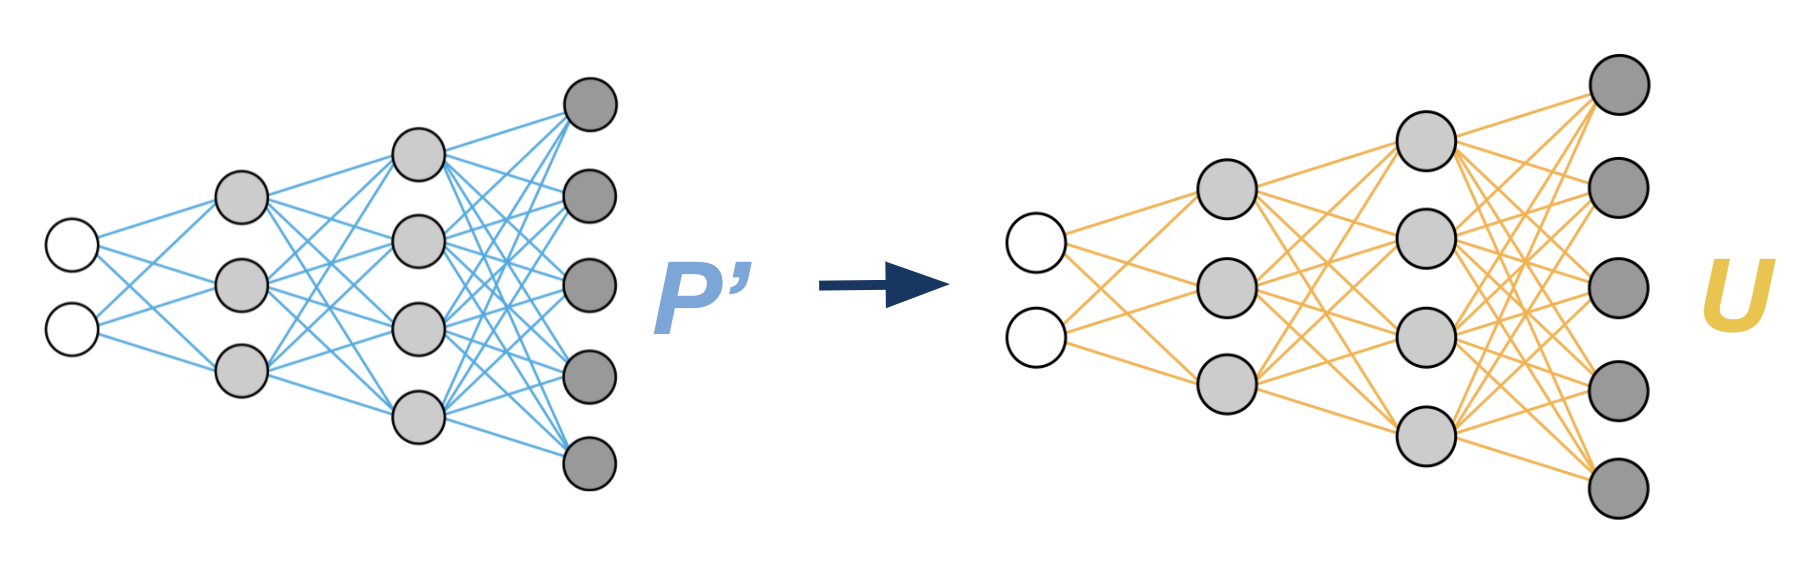
\includegraphics[width=1\textwidth]{figures/c6_active_div/diagrams/divergent_finetuning.png}
    \caption[Diagram illustrating the network parameter view of divergent fine-tuning.]{Diagram illustrating the network parameter view of divergent fine-tuning. A network pre-trained on the distribution $P$ and can produce the approximate distribution \textcolor{blue}{$P'$} is fine-tuned in a divergent fashion to create a novel distribution \textcolor{orange}{$U$}.}
  \label{fig:c6:divergent-finetuning}
  \end{figure}

\subsubsection{Cross-Domain Training} 

In cross-domain training, transfer learning is performed to a pre-trained model that generates the approximate distribution $P'$ and is then trained to approximate the new data distribution $Q$. 
This transfer learning procedure will eventually lead to the model learning a set of parameters that generate the approximate distribution $Q'$. 
However, by picking an iteration of the model mid-way through this process, a set of parameters can be found that produced a blend between the two approximate distributions $P'$ and $Q'$, resulting in the producing the novel distribution $U$ \citep{schultz2020mixed}. 
This method was discovered by many artists and practitioners independently, who were performing transfer learning with GAN models for training efficiency, but noted that the iterations of the model part-way through produced the most interesting, surprising and sometimes horrifying results \citep{adler2020transfer,black2020noface,mariansky2020transfer,shane2020cat}.

\begin{figure}[!htbp]
    \centering
    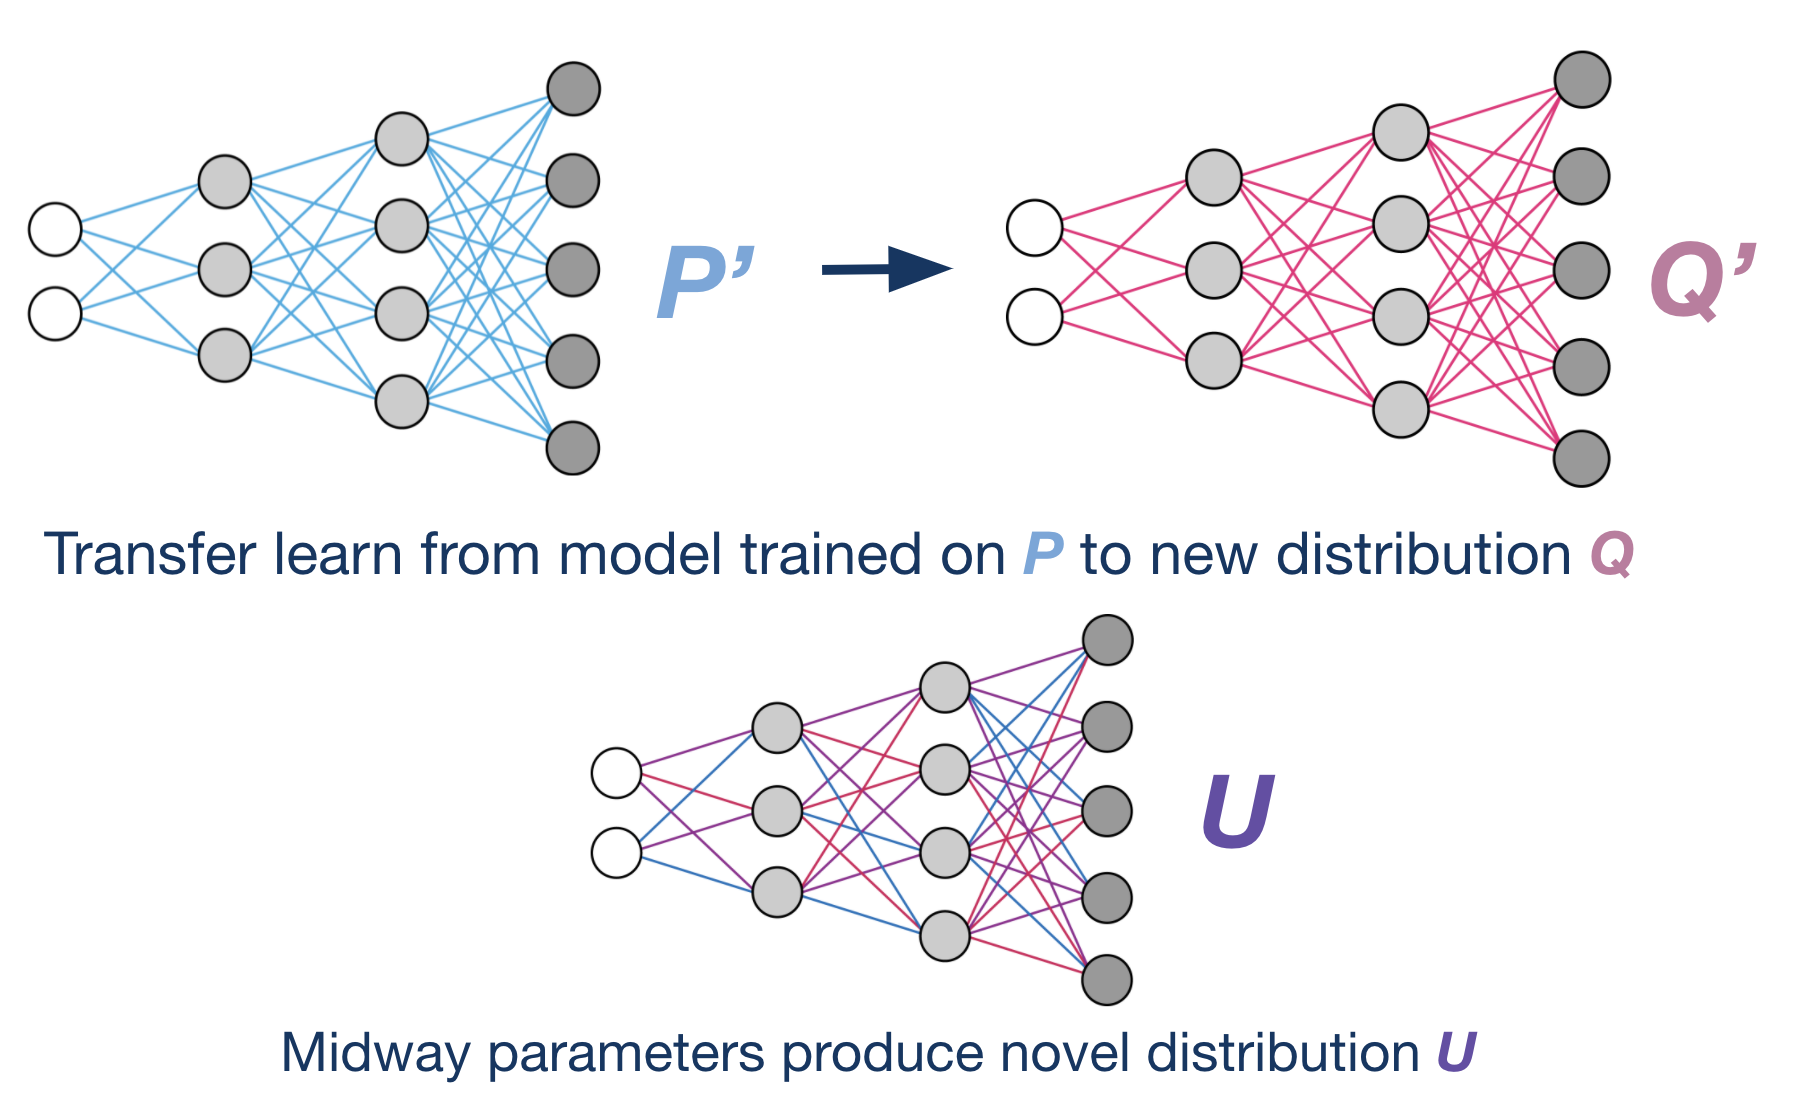
\includegraphics[width=1\textwidth]{figures/c6_active_div/diagrams/cross_domain_training.png}
    \caption[Diagram illustrating the network parameter view of cross-domain training.]{Diagram illustrating the network parameter view of cross-domain training. A network pre-trained on the distribution $P$ that produces the approximate distribution \textcolor{blue}{$P'$} is used as the starting point for transfer learning to a new distribution $Q$ that will eventually learn to produce the approximate distribution \textcolor{magenta}{$Q'$}. If early stopping is performed through the transfer learning process, a set of parameters for the network that produces the novel hybrid distribution \textcolor{violet}{$U$} can be ascertained.}
  \label{fig:c6:cross-domain-training}
  \end{figure}

\subsubsection{Continual Domain Shift}
\label{section:domainshift}

Going beyond simply mixing two domains, one approach that gives more opportunity to steer the resulting distribution in the fine-tuning procedure, is to optimise on a domain that is continually shifting. In creating the artworks \textit{Strange Fruit} \citep{som2020strange}, the artist Mal Som ``iterate[s] on the dataset with augmenting, duplicating and looping in generated images from previous ticks'' to steer the training of the generator model \citep{som2021personal}. 
In this process, the target distribution $Q_t$ at step $t$ may contain samples $q'_{t-n}$ generated from earlier iterations of the model at any previous time step $t-n$ where $0<n<t$. 
Additionally, the target distribution $Q_t$, may no longer include samples or may have duplicates of samples $q_{t-n}$ from previous iterations of the target distribution. 
Using this process, the target distribution can be continually shaped and guided. 

This process of modelling a continually shifting domain often leads to the ---generally unwanted--- phenomenon of mode collapse \citep{thanh2020catastrophic}. 
However, in Som's practice, this is induced deliberately. After a model has collapsed, Som explores its previous iterations to find the last usable instance right before collapse. 
Som likens this practice to the artistic technique of defamiliarisation, where common things are presented in unfamiliar ways so audiences can gain new perspectives and see the world differently \citep{som2021personal}.

Som's artistic experiments are a precursor to subsequent research studies that demonstrate that generative models that are subsequently trained on their own synthetic outputs, regularly lead to mode (or model) collapse \citep{alemohammad2023self, martinez2023combining, shumailov2023curse, shumailov2024ai}. An issue that is becoming so widespread, with the outputs of generative AI polluting the internet with `low-quality' data, that the issue has even made its way into the popular and business press \citep{peel2024problem,aatish2024threat}.

\subsubsection{Loss Hacking} 

An alternative strategy is to fine-tune a model without any training data. 
Instead, a loss function is used that directly transforms the approximate distribution $P'$ into a novel distribution $U$ without requiring any other target distribution. 
Chapter \ref{ch:divergent} uses the frozen weights of the discriminator to directly optimise away from the likelihood of the data, by using the inverse of the adversarial loss function. 
This process reverses the normal objective of the generator to generate `real' data and instead generates samples that the discriminator deems to be `fake'. 
By applying this process to a GAN that can produce photo-realistic images of faces, this fine-tuning procedure crosses the uncanny valley in reverse, taking images indistinguishable from real images, and amplifying the uncanniness of the images before eventually leading to mode collapse. 
In a similar fashion to Som's practice (see previous sub-section), one instance of the model before mode collapse was hand-selected and a selection of its outputs turned into the series of artworks \textit{Being Foiled} \citep{broad2020being} (\S \ref{c7:sec:divergent}).

\subsubsection{Infusing External Knowledge} 

By harnessing the learned knowledge of externally trained models, it is possible to fine-tune models to infuse that knowledge to transform the original domain data with characteristics defined using the auxiliary model. 
In \citep{broad2019transforming}, I utilised a classifier model $C_{classifier}$ trained to differentiate between datasets, in conjunction with the frozen weights of the discriminator $D_{frozen}$ to fine-tune a pre-trained GAN generator model $G$ away from the original distribution and towards a new local minimum defined by the loss function $L$.\footnote{Whilst this work was done during the course of my PhD research, it has been left out of the final writeup of this thesis for two reasons: the work was not peer-reviewed in a published conference (only being disseminated as an arxiv pre-print), and the work is not strictly data-free, the common thread between the three experimental contributions presented in Chapters \ref{ch:unstable_eq}, \ref{ch:divergent} \& \ref{ch:net_bend}.}
$L$ is defined as the weighted sum of the two auxiliary models $L = \alpha C_{classifier}(G(x)) + \beta D_{frozen}(G(x))$ given the random latent vector $x$, and $\alpha$ and $\beta$ being the hyper-parameters defining the weightings for the two components of the loss function. 

The StyleGAN-NADA framework \citep{gal2021stylegan} takes advantage of the external knowledge of a contrastive language–image pre-training model (CLIP) \citep{radford2021learning}. 
CLIP has been trained on billions of text and image pairs from the internet and provides a joint-embedding space of both images and text, allowing for similarity estimation of images and text prompts. 
In StyleGAN-NADA, pretrained StyleGAN2 models \citep{karras2019analyzing} can be fine-tuned using user-specified text prompts, the CLIP model $C_{clip}$ is then used to encode the text prompts and the generated samples in order to provide a loss function where the cosine similarity $S$ between the clip encodings of the text string $t$ and the generated image embedding $G(x)$ given random latent $x$, can be minimised using the loss $L = S(C_{clip}(t), C_{clip}(G(x))$. 
This training procedure guides the generator towards infusing characteristics from an unseen domain defined by the user as text prompts.

\subsubsection{Reinforcement Learning from Human Feedback} 

Reinforcement learning from human feedback (RLHF) is an approach to fine-tuning models not using new training data, but by using human feedback to both label and correct the outputs of generative models \citep{ziegler2019fine}. 
This approach is most commonly used in the alignment of large language models (LLMs) (\S \ref{c6:subsec:alignment}), where unwanted outputs derived from the original training data are corrected, and the outputs of the generative neural networks are more closely `aligned' with specified human values, which is a common issue when models are trained on mass scraped data from the internet which contains many unwanted outputs, such as racist, misogynistic or things that could be considered dangerous.
Whilst RLHF is a means by which models are fine-tuned to diverge from their original training data distributions, it is still primarily an \textbf{imitation-based} form of learning.
Whilst it could be used to fine-tune models in a truly divergent fashion (discussed in the future research directions \S \ref{c6:subsec:divergent-rlhf}), for now, it is primarily used as a form of imitation learning to correct and align the outputs generative models.

\subsection{Chaining models}
\label{survey:chaining}

An approach that is widely used by artists who incorporate generative models into their practice, but not well documented in academic literature, is the practice of chaining multiple custom models trained on datasets curated by the artists. 
The ensembles used will often utilise standard unconditional generative models, such as GANs, in combination with other conditional generative models such as image-to-image translation networks, such as pix2pix \citep{isola2017image} and CycleGAN \citep{zhu2017unpaired}, along with other approaches for altering the aesthetic outcomes of results such as style transfer \citep{gatys2016neural}. 
Artists will often train many models on small custom datasets and test out many combinations of different models, with the aim of finding a configuration that produces unique and expressive results. 
The artist Helena Sarin will often chain multiple CycleGAN models into one ensemble, and will reuse training data during inference, as the goal of this practice ``is not generalization, my goal is to create appealing art'' \citep{sarin2018playing}. 
The artist Derrick Schultz draws parallels between the practice of chaining models and Robin Sloan's concept of `flip-flopping' \citep{schultz2021personal}, where creative outcomes can be achieved by ``pushing a work of art or craft from the physical world to the digital world and back, often more than once'' \citep{sloan2012flipflop}.
An example of Schultz's work, where network bending is used as part of chaining models, is detailed in \S \ref{c7:subsubsec:schultz}.


\subsection{Network Bending}
\label{survey:bending}

\begin{figure}[!htbp]
    \centering
    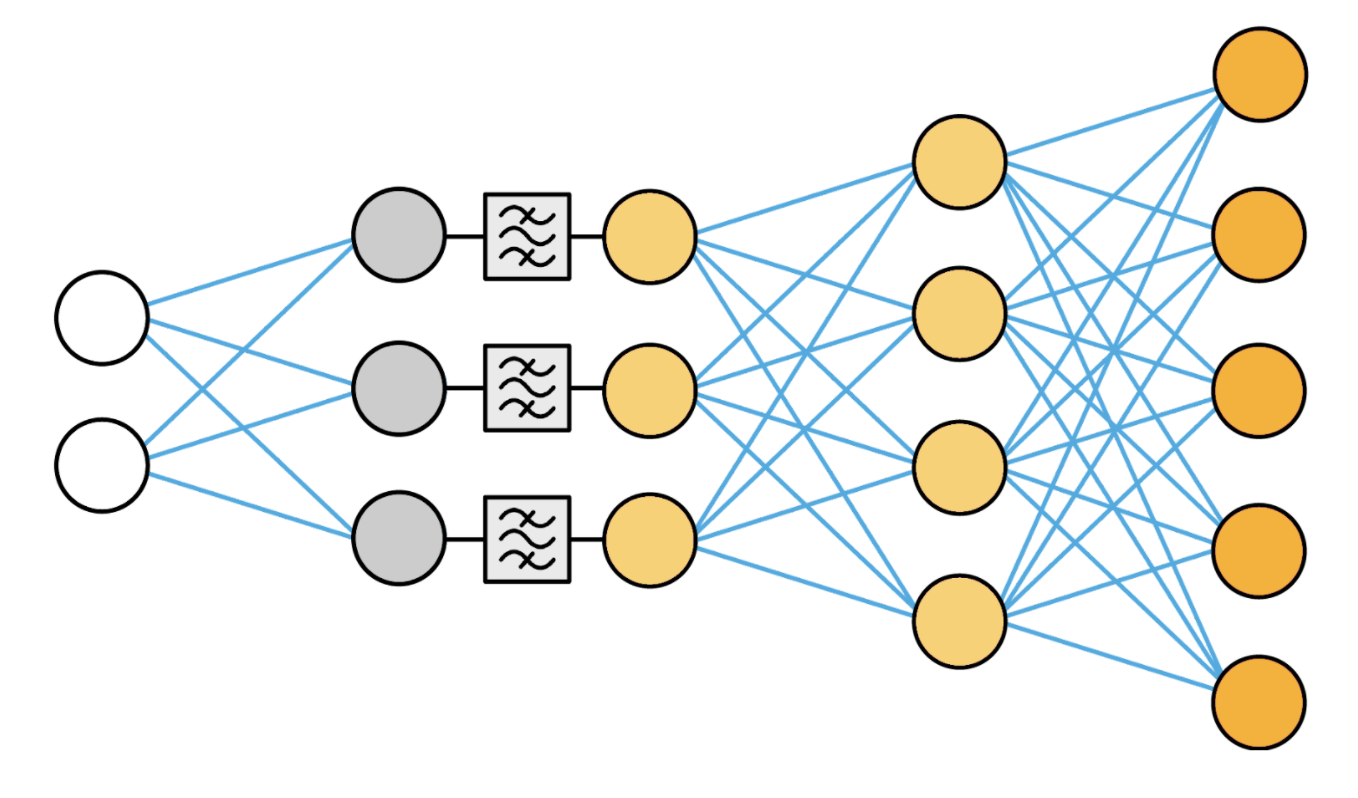
\includegraphics[width=1\textwidth]{figures/c6_active_div/diagrams/network_bending.png}
    \caption[Diagram illustrating the network parameter view of network bending.]{Diagram illustrating the network parameter view of network bending. A network pre-trained on the distribution $P$ that produces the approximate distribution \textcolor{blue}{$P'$} has additional deterministic transform layers inserted into it which when activated are used to produce the novel distribution \textcolor{orange}{$U$}.}
  \label{fig:c6:network-bending}
  \end{figure}

Network bending \citep{broad2021network,broad2022network} (presented in Chapter \ref{ch:net_bend}) is a framework that allows for active divergence using individual pre-trained models without making any changes to the weights or topology of the model. 
Instead, additional layers that implement standard image filters are inserted into the computational graph of a model and applied during inference to the activation maps of the convolutional features\footnote{
    Inserting filters into GANs was also developed independently in the Matlab StyleGAN playground \citep{pinkney2020matlab}.}. 
As the computational graph of the model has been altered, the model which previously generated samples from the approximate distribution $P'$, now produces novel samples from the new distribution $U$, without any changes being made to the parameters of the model. 
In the simplest case of a two-layer model an association weight matrix $W_l$ and bias $b_l$ vector for each layer $l$. 
Which generates sample $p'=\sigma(W_2(\sigma(W_1x+b_1))+b_2)$ from input vector $x$ and using a non-linear activation function $\sigma$. 
In the network bending framework, a deterministic function $f$ (controlled by the parameter $y$) is inserted into the computational graph of the model and applied to the internal activations of the model $u=\sigma(W_2(f(\sigma(W_1x+b_1),y))+b_2)$, allowing the model to produce new samples $u$ from the new distribution $u \in U$. Beyond the simplest case of a transformation being applied to all features in a layer, the transformation layer can also be applied to a random sub-section of features, or to a pre-selected set of features (\S \ref{c5:sec:clustering}). 

Network bending has been further developed by others into applications in other forms of generative models and domains, as well as building user interfaces for network bending.
A full account of the technical impact of the network bending work is given in \S \ref{c7:sec:net-bend-impact}.

\subsection{Network Blending}
\label{survey:blending}

Blending multiple models trained on different datasets allows for more control over the combination of learned features from different domains. 
This can either be done by blending the predictions of the models, or by blending the parameters of the models themselves.

\subsubsection{Blending Model Predictions} 

\citet{akten2016real} present an interactive tool for text generation allowing for the real-time blending of the predicted outputs of an ensemble of long-short term memory network (LSTM) models \citep{hochreiter1997long} trained to perform next character prediction from different text sources. 
A graphical user interface allows the user to dynamically shift the mixture weights for the weighted sum for the predictions of all of the models in the ensemble, prior to the one hot vector encoding which is used to determine the final predicted character value.


\subsubsection{Blending Model Parameters} 
A number of approaches, all demonstrated with StyleGAN2 \citep{karras2019analyzing}, take advantage of the large number of pre-trained models that have been shared on the internet \citep{pinkney2020awesome}. 
Of these, almost all have been transfer-learned from the official model weights trained on the Flickr-Faces High Quality (FFHQ) dataset.
It has been shown that the parameters of models transfer-learned $p_{transfer}$ from the same original source $p_{base}$ share commonalities in the way their weights are structured. 
This makes it possible to meaningfully interpolate between the parameters of the models directly \citep{aydao2020interp}. 
By using an interpolation weighting $\alpha$, it is possible to control the interpolation for the creation of a set of parameters $p_{interp} = (1 - \alpha)p_{base} + \alpha p_{transfer}$. 

\begin{figure}[!htbp]
    \centering
    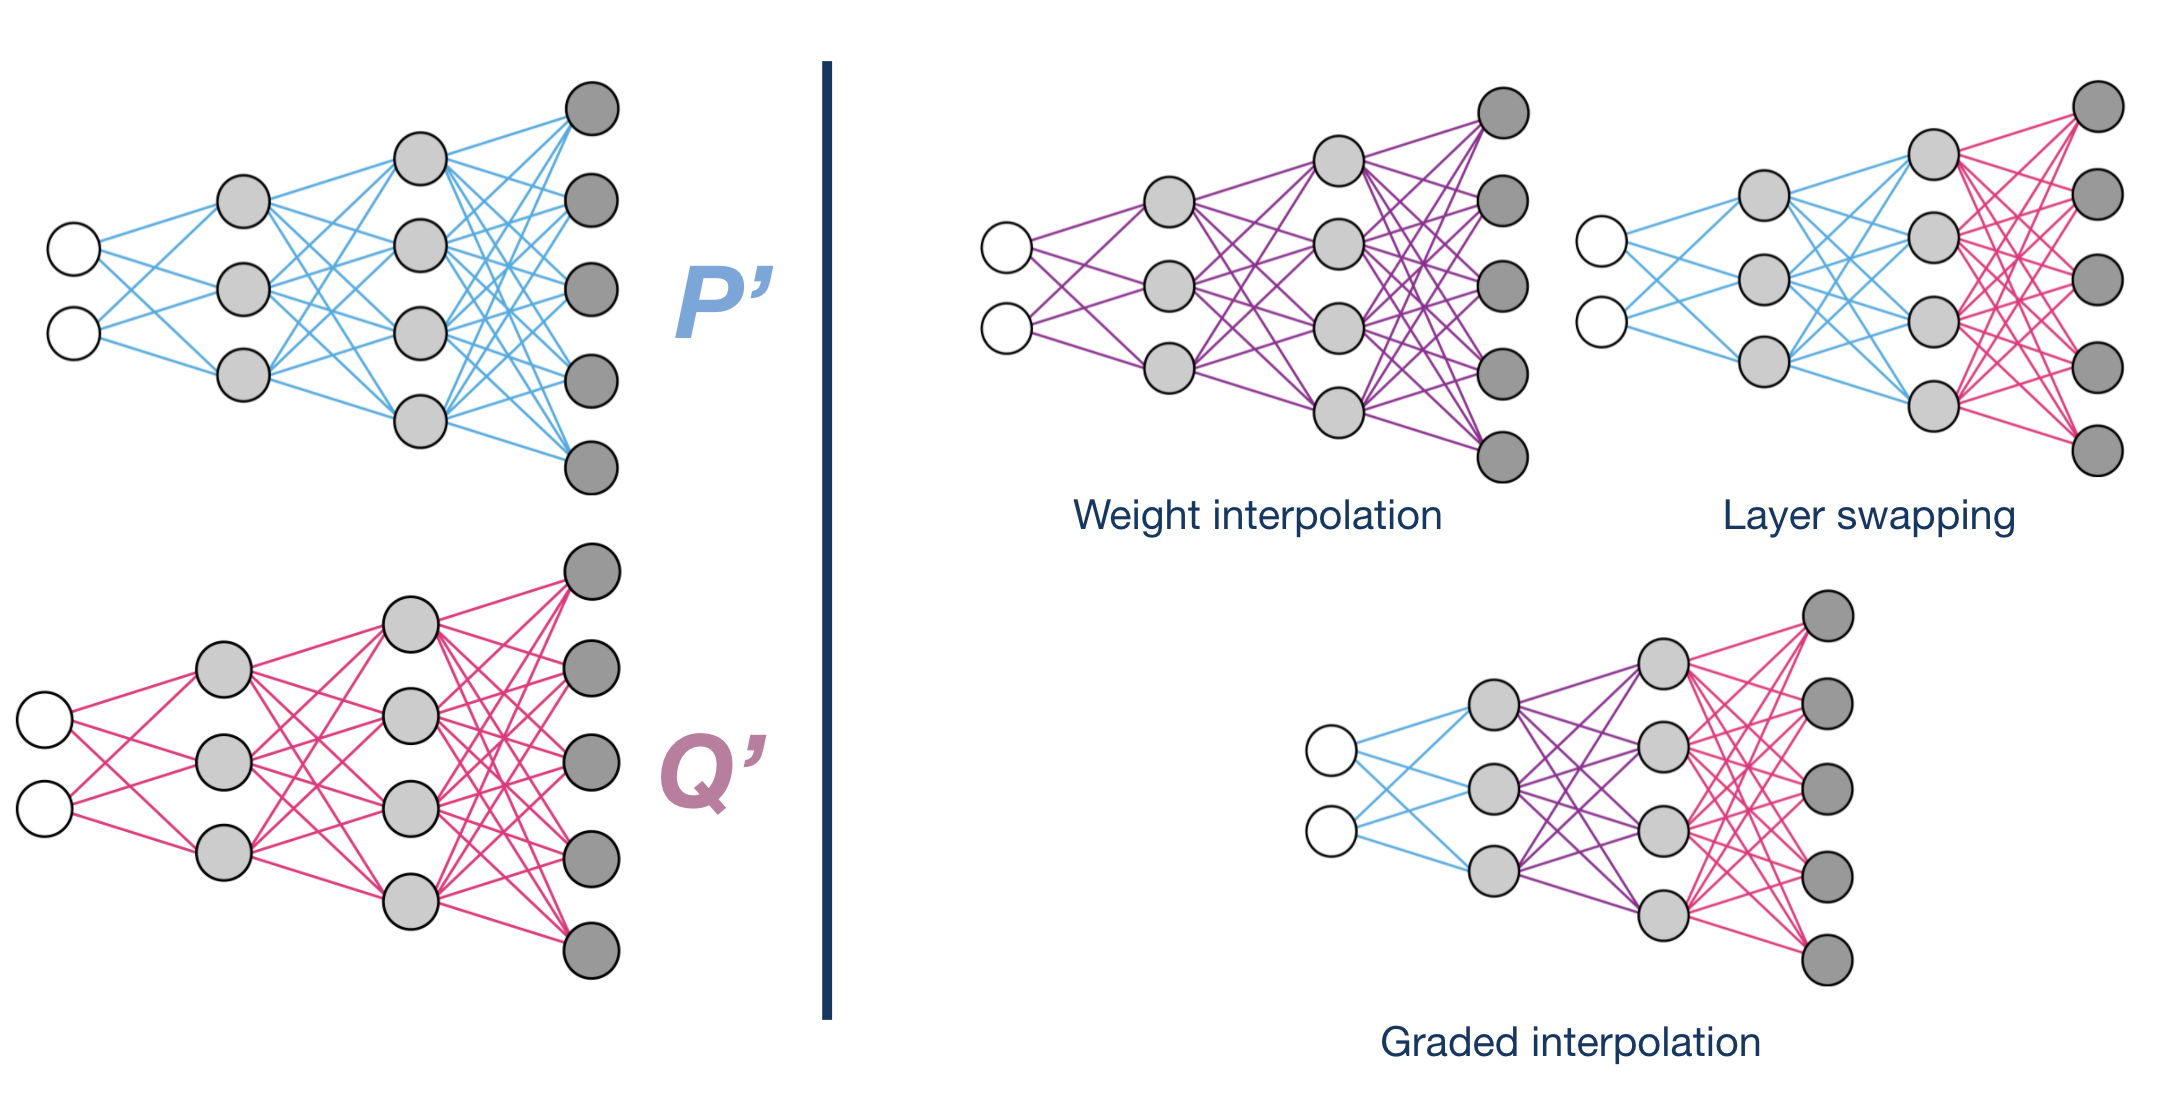
\includegraphics[width=1\textwidth]{figures/c6_active_div/diagrams/network_blending.png}
    \caption[Diagram illustrating the network parameter view of network blending.]{Diagram illustrating the network parameter view of network blending. Two networks, pre-trained on the distributions $P$ and $P$ that then produce the approximate distributions \textcolor{blue}{$P'$} and \textcolor{magenta}{$Q'$} can have their parameters blended by either interpolating on the weights, swapping the layers between models or performing graded interpolation across the model hierarchy.}
  \label{fig:c6:network-blending}
  \end{figure}

Layers can also be swapped from one model to another \citep{pinkney2020interpolation}, allowing the combination of higher-level features of one model with lower-level features of another. 
This layer-swapping technique was used to make the popular `toonification' method, which can be used to find the corresponding sample to a real photograph of a person in a Disney-Pixar-esque `toonified' model, simply by sampling from the same latent vector that has been found as the closest match to the person in FFHQ latent space \citep{abdal2019image2stylegan}. 
A generalised approach that combines both weight interpolation and layer-swapping methods for multiple models, uses a cascade of different weightings of interpolation for the various layers of the model \citep{arfafax2020barycentricnotebook}.

\citet{colton2021evolving} presents an evolutionary approach for exploring and finding effective and customisable neural style transfer blends. 
Upwards of 1000 neural style transfer models trained on 1-10 style images each can be blended through model interpolation, using an interface that is controlled by the user. 
MAP-Elites \citep{mouret2015illuminating} in combination with a fitness function calculated using the output from a ResNet model \citep{he2016deep} were used in evolutionary searches for optimal neural style transfer blends. 

\subsection{Model Rewriting}
\label{survey:rewriting}

Model rewriting encompasses approaches where either the weights or network topology are altered in a targeted way, through manual intervention or by using some form of heuristic-based optimisation algorithm. 

\subsubsection{Stochastic Rewriting} 

To create the series of artworks \textit{Neural Glitch} the artist Mario Klingemann randomly altered, deleted or exchanged the trained weights of pre-trained GANs \citep{klingemann2018neural}. 
In a similar fashion, the convolutional layer reconnection technique \citep{ruzika2020gan} randomly swaps convolutional features within layers of pre-trained GANs. 
This technique is applied in the \textit{Remixing AIs} audiovisual synthesis framework \citep{collins2020remixing}.

\subsubsection{Targeted Rewriting} 
\citet{bau2020rewriting} presents a targeted approach to model rewriting. 
Here, a sample is taken from the model and manipulated using standard image editing techniques (referred to as a `copy-paste' interface). 
Once the sample has been altered corresponding to the desired goal (such as removing watermarks from the image or getting horses to wear hats), a process of constrained optimisation is performed. 
All of the layers but one are frozen, and the weights of that layer are updated using gradient descent optimisation until the generated sample matches the new target. 
After this optimisation process is complete, the weights of the model are modified such that the targeted change becomes present in all the samples that the model generates.

\begin{figure}[!htbp]
    \centering
    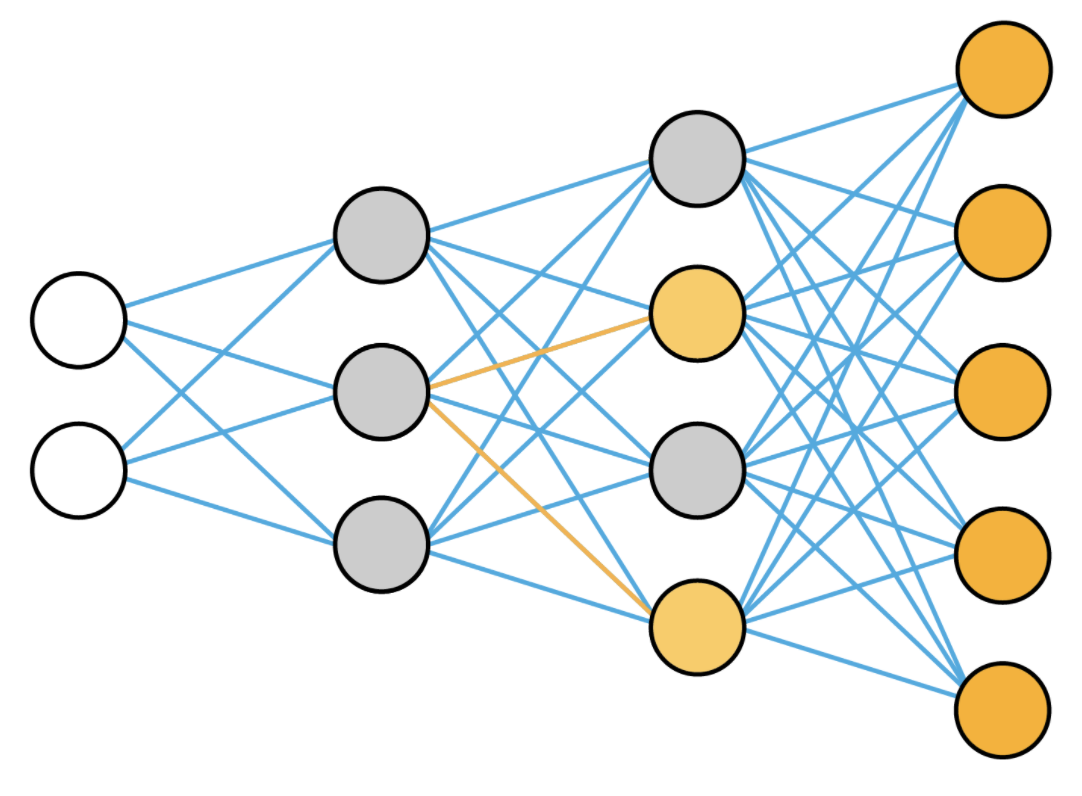
\includegraphics[width=1\textwidth]{figures/c6_active_div/diagrams/model_rewriting.png}
    \caption[Diagram illustrating the network parameter view of model rewriting.]{Diagram illustrating the network parameter view of model rewriting. A network pre-trained on the distribution $P$ that produces the approximate distribution \textcolor{blue}{$P'$} has selected changes made to a small number of parameters resulting in the new distribution \textcolor{orange}{$U$}.}
  \label{fig:c6:model-rewriting}
  \end{figure}

The CombiNets framework \citep{guzdial2018combinets}, informed by prior research in combinational creativity \citep{boden2004creative}, can be utilised to create a new model by combining parameters from a number of pre-trained models in a targeted fashion. 
The parameters of existing models are recombined to take into account a new mode of generation that was not present in the training data (an example given would be a unicorn for a model trained on photographs of non-mythical beings). 
In this framework, a small number of new samples is provided (not enough to train a model directly) and then heuristic search is used to recombine parameters from existing models to account for this new mode of generation.
As this approach aims to rewrite the parameters of two or more models together, it could also be considered a form of \textit{network blending} (\S \ref{survey:blending}).

\section{Further Demarcations of Active Divergence Methods}

\subsection{Training from Scratch vs. Using Pretrained Models}

Finding stable, effective ways of training generative models, in particular GANs, is difficult and, depending on the training scheme, there are only a handful of methods that have been found to work successfully. Few methods for active divergence train a model completely from scratch. Instead, most take pre-trained models as their starting point for interventions. This way, training from scratch can be avoided, but fine-tuning may still be required. 


\subsection{Utilising Data vs. Data-Free Approaches}
\label{c6:subsec:datafree}

Most of the approaches described utilise data in some way, whether as an inspiring set for novelty generation or for combining features from different datasets (divergent fine-tuning, network blending and chaining models). 
Even methods for model rewriting use very small amounts of example data to guide optimisation algorithms that alter the model weights. 
However, methods like network bending, show how models can be analysed in ways that don't rely on any data, and are used for intelligent manipulation of the model's --- an approach which could be applied to other methods like model rewriting. 
Methods that train and fine-tune models without data also show how auxiliary networks and the dynamics between models can be utilised for achieving active divergence.
The common thread of the novel technical contributions in this thesis (presented in Chapters \ref{ch:unstable_eq}, \ref{ch:divergent} \& \ref{ch:net_bend}) are all data-free approaches to active divergence.

\subsection{Human Direction vs. Creative Autonomy}
Very few of the approaches described have been developed with the expressed intention of handing over creative agency to the systems themselves. Most of the methods have been developed by artists or researchers in order to allow people to manipulate, experiment with and explore the unintended uses of these models for creative expression. However, the methods described that are currently designed for, or rely on a high degree of human curation and intervention, could easily be adapted and used in co-creative or autonomous creative systems in the future \citep{berns2021automating}.

\section{Related Research Areas}
\label{c6:sec:related-research}

Since the publication of the original survey paper \citep{broad2021active}, there have been two areas of related research in generative neural networks that have emerged to be significant sub-fields of AI research, that are considered related fields or even subfields of active divergence research. 

\subsection{Alignment}
\label{c6:subsec:alignment}

AI alignment first emerged from the philosophical study of AI, which focuses on AI safety, and the goal of ensuring that the behaviour of AI `aligns' with human values \citep{yudkowsky2016ai, gabriel2020artificial}. 
The first attempts at codifying rules for AI agents were made much earlier than the current discourse around AI alignment, and examples from science fiction literature such as Asimov's Three Laws of Robotics \citep{asimov1942runaround}, can be considered constituting the first proposed ways that the behaviour of AI is governed, or aligned with human values. 

How `human-values' are defined, is not always universally agreed upon \citep{turchin2019ai}. 
Often, when done by large organisations, alignment is driven as much by legal compliance, liability, and the avoidance of public relations controversies, as it is defined by a universally agreed-upon set of human values. 

\cite{ji2023ai} gives a comprehensive account survey of methods for achieving AI alignment, which is most commonly done in the space of large language models based on transformer architectures \citep{vaswani2017attention}. 
The most commonly used method for alignment is Reinforcement Learning from Human Feedback (RLHF) \citep{ziegler2019fine}, which is used by many companies now that provide LLMs as API services. 
RLHF could be considered a form of \textit{divergent fine-tuning} (\S \ref{survey:divergent}), though this is often done to imitate human preferences and to prevent LLMs from repeating racist, misogynistic or generating other dangerous outputs that would have been learnt from original training data (usually on text mass-scraped from the world wide web).
So while this is diverging from the original training data, this is usually still done as a form of imitation-based learning in the fine-tuning stage.

\subsection{Data Poisoning}

Data poisoning, first performed by \cite{biggio2012poisoning}, is the task of injecting data into training datasets that interfere with the training and optimisation process for malicious effect \citep{fan2022survey}. 
Data poisoning has become popular in the generative space with widely used algorithms such as \textit{glaze} \citep{shan2023glaze} \textit{nightshade} \citep{shan2024nightshade}, which are designed to protect the intellectual property of artists against their work being used without consent in training text-to-image diffusion models \citep{rombach2022high}. 
In this context, data poisoning for generative models can be seen as an approach to active divergence where the data is deliberately corrupted in order to prevent the faithful imitation of the training data and disrupt training such that the generative model no longer accurately models the training data, but instead, diverges from it in unwanted ways (from the perspective of the actors who are training the generative model). 

\section{Applications of Active Divergence}

In this section, I outline some of the applications for active divergence methods outside of the two related areas of research detailed in the previous section (\S \ref{c6:sec:related-research}).

\subsection{Novelty generation}

Generative deep learning techniques are capable of generalisation, such that they can produce new artefacts of high typicality and value, but are rarely capable of producing novel outputs that do not resemble the training data. Active divergence techniques play an important role in getting generative deep learning systems to generate truly novel artefacts, especially when there may be limited or even no data to draw from. 

\subsection{Creativity Support and Co-Creation}

Some of the frameworks presented are already explicitly designed as creativity support tools, such as the network bending framework, designed to allow for expressive manipulation of deep generative models. The \textit{Style Done Quick} \citep{colton2021evolving} application where many style transfer models have been evolved, was built as a casual creator application \citep{compton2015casual}. Though many of the other methods described are still preliminary artistic and research experiments, there is a lot of potential for these methods to become better understood and eventually adapted and applied in more easily accessible creativity support tools and co-creation frameworks. 

\subsection{Knowledge Recombination}

Reusing and recombining knowledge in efficient ways is an important use-case of active divergence methods. While impressive generalisation can be ascertained from extremely large models trained on corpora extracted from large portions of the internet \citep{ramesh2021zero}, this is out of the capabilities for all but a handful of large tech companies. Instead of relying on ever-expanding computational resources, active divergence methods allow for the recombination of styles, aesthetic characteristics and higher-level concepts in a much more efficient fashion. Methods like chaining models, network blending and model rewriting offer alternatives routes to achieving flexible knowledge recombination and generalisation to unseen domains without the need for extremely large models or data sources. 


\subsection{Unseen Domain Adaptation}

Active divergence methods allow for the possibility of adapting to and exploring unseen domains, for which there is little to no data available. The network blending approach presented by \citet{pinkney2020interpolation} can be used for the translation of faces while maintaining recognisable identity into a completely synthesised data domain, something which would not be possible with standard techniques for image translation \citep{zhu2017unpaired}.

The model rewriting and network bending approaches offer the possibility of reusing and manipulating existing knowledge in a controlled fashion to create new data from a small number of given examples, or theoretically without any prior examples if external knowledge sources are integrated, as discussed further below. This approach could also be utilised by agents looking to explore hypothetical situations, by reorganising learned knowledge from world models \citep{ha2018worldmodels} to explore hypothetical situations or relations. 

\section{Future Research Directions}
\label{c6:sec:future}

In this section, I discuss possible future research directions and applications for developing, evaluating and utilising methods for active divergence.

\subsection{Metrics for Quantitative Evaluation}

For the advancement of research on active divergence, methods for quantitative evaluation will be critical in order to keep track of progress, to compare techniques and for benchmarking. Metrics for active divergence will have to go beyond measuring the similarity or dissimilarity between distributions, as is usually done in the evaluation of generative models \citep{gretton2019interpretable}. Active divergence metrics should contribute to a better understanding of \textit{how} the distributions diverge. Therefore, various changes to the modelled distribution should be taken into consideration when looking to measure divergence between distributions in creative contexts. These include increases or decreases in diversity, the consistency and concurrency of change across the whole distribution and whether changes primarily affect low or high-level features.

\subsection{Automating Qualitative Evaluation}

In addition to quantitative evaluation, other metrics are needed for evaluating active divergence metrics. In order to rely less on qualitative evaluation for guiding decisions in creating new models, and do this in computational fashion so that these aspects of the process can be handed over to the computational systems. For instance, a recently developed metric for measuring visual indeterminacy \citep{wang2020towards}, which is argued as being one of the key drivers for what people find interesting in GAN-generated art \citep{hertzmann2020visual}, could be used for replacing the qualitative evaluation and curation step done by humans. Other metrics that could be used are novelty metrics \citep{grace2019expectation}, bayesian surprise \citep{itti2009bayesian}, aesthetic evaluation \citep{galanter2012computational}, or measurements for optimal blends between data domains and evaluating the novelty of changes made to semantic relationships.

\subsection{Inventing New Objective Functions}

None of the methods presented to date that are based on generative deep learning have been capable of inventing their own objective functions. Instead, methods such as creative adversarial networks \citep{elgammal2017can} rely on hand-crafted variations of well-established objective functions. This will be one of the most challenging future research directions to overcome, as generative deep learning systems rely on a small handful of objectives that result in stable convergence. However, in conjunction with the development of new evaluation metrics, it may be possible to explore whole new categories of objective functions that diverge from existing data representations and produce artefacts of high value. 

\subsection{Utilising External Knowledge}
\label{future:external}
Harnessing expert knowledge external to the dataset, which may come from separate domains or symbolic knowledge representations will allow much more flexibility in how generative models are manipulated in combinational creativity \citep{boden2004creative} and conceptual blending frameworks \citep{fauconnier2008way}. Combining research into analysing the semantic purpose and relationship between features, and creating mappings of those to external data sources or knowledge graphs, would allow for more flexibility in controlling techniques which currently rely on human intervention (network bending, model rewriting).

\subsection{Multi-Agent Systems}

It has been argued that the GAN framework is the simplest example of a multi-agent system \citep{arcas2019social}, and frameworks such as neural cellular automata \citep{mordvintsev2020growing} offer new possibilities for multi-agent approaches in generative deep learning. The active divergence methods for training without data described in this paper all rely on the dynamics of multiple agents to produce interesting results, but this could be taken much further. It has been argued that art is fundamentally social \citep{hertzmann2021social} and exploring more complex social dynamics between agents \citep{saunders2019multi} could be a fruitful avenue for exploration in the development of these approaches. There is a large body of work in emergent languages from cooperative multi-agent systems \citep{lazaridou2016multi} that could be drawn from in furthering the work in generative multi-agent systems. 

\subsection{Open-Ended Reinforcement Learning}
\label{c6:subsec:open-ended}

Open-ended reinforcement learning, where there is no set goal \citep{wang2020enhanced}, offers possibilities for new more autonomous approaches to achieving active divergence. Reinforcement learning has not been discussed in this survey, but has been used in generative settings \citep{luo2020reinforcement} in nascent research. Reinforcement learning approaches offer many opportunities for frameworks of creativity to be explored that are not available to standard generative deep learning methods, as they take actions in response to their environment, rather than just fitting functions. Paradigms like intrinsic motivation \citep{shaker2016intrinsically}, cooperating or competing with other agents, and formulating and acting on intentions are all concepts that conventional generative deep learning systems alone cannot explore, but these paradigms could be explored in open-ended systems utilising reinforcement learning.

\subsection{Divergent RLHF}
\label{c6:subsec:divergent-rlhf}

RLHF is most commonly used as a form of imitation-based learning in order to correct and align the outputs of large models, such as LLMs and text-to-image models. 
However, this is not the only possible use for this.
For instance, RLHF could be used for more personalised divergent fine-tuning of models, to actively fine-tune towards novel data distributions, and more closely align to an individual's aesthetic preferences. 
Using RL to fine-tune generative neural networks could also be used in conjunction with open-ended RL (\S \ref{c6:subsec:open-ended}) to fine-tune models in truly novel and divergent directions. 

\section{Conclusion}

This chapter has presented a comprehensive survey of active divergence methods, as well as related areas of research and potential future research directions for active divergence research. 
Active divergence has been the primary goal of all of the research in this thesis, even if it was done primarily before the term active divergence was conceived in 2020. 
The research in this thesis constitutes three categorical contributions to active divergence methods: \textit{training without data} (Ch. \ref{ch:unstable_eq}; \S \ref{survey:nodata}), \textit{divergent fine-tuning} (Ch. \ref{ch:divergent}; \S \ref{survey:divergent}), and \textit{network bending} (Ch. \ref{ch:net_bend}; \S \ref{survey:bending}). 
All of the methods I have presented in this thesis as original research contributions are data-free (\S \ref{c6:subsec:datafree}), which makes this a largely unique and novel approach to achieving active divergence. 
These contributions, along with the formal technical delineation and survey of methods presented in this chapter make up to distinct contributions of research in this thesis.
The following chapter (Ch. \ref{ch:impact}) details the artistic and technical impact of my work outside of the formal active divergence perspective presented in this chapter. 
